\chapter{Probability Distributions \label{chapter:probabilitydistributions}}

Many of the methods we will examine in these workshops depend on basic concepts from probability theory. For example, linear and logistic regression are members of a class of supervised learning algorithms called \textbf{generalized linear models} (see Chapter~\ref{chapter:glms}) which make assumptions about the type of probability distribution followed by the outcome variable. Decision trees use a concept called \textbf{entropy} (see Chapter~\ref{chapter:decisiontrees}), whose mathematical formulation depends on the probability distribution underlying the outcome. Many \textbf{hypothesis tests} (see Chapter~\ref{chapter:hypothesistesting}) likewise rely on probabilistic assumptions about the data. Probability is everywhere.

The following sections review some key probability concepts -- in an extremely hand-wavey and non-rigorous way -- and the properties of some of the most common probability distributions you will encounter in machine learning and statistics. 

\section{Definitions}

A \textbf{probability distribution} is just a mathematical function that provides the relative likelihoods of various possible outcomes of an observation. We call the quantity that is being observed a \textbf{random variable}. Probability distributions can be discrete or continuous. The random variable involved can be a number, a vector of numbers, a category/class, etc. The \textbf{sample space} is the set of all possible outcomes. The integral (or sum) of the probability distribution over the entire sample space is $1.0$. You will often hear probability distributions for continuous random variables referred to as \textbf{probability densities}. 

Probability distributions are grouped into families that are characterized by their overall shapes. These families contain \textbf{parameters} that, when varied, produce different distributions. Specific probability distributions from within a single family can often look quite different. 

We use the notation $E[x|\theta]$ to refer to the \textbf{expected value}, or mean, of a distribution, given its parameter(s), $\theta$. There can be more than one parameter, and it will not always be called $\theta$; this is just an example. We use the notation $\text{var}(x|\theta)$ to refer to the \textbf{variance}, or spread, of a distribution around its mean. 

\section{Normal Distribution} 

Also called the \textbf{Gaussian distribution}, the normal distribution is probably the most well-known continuous probability distribution. It has the following properties:
\begin{equation*} p(x | \mu, \sigma) = \frac{1}{\sqrt{2 \pi \sigma^2}} e^{-\frac{(x-\mu)^2}{2 \sigma^2}} \qquad  E[x| \mu, \sigma] = \mu \qquad \text{var}(x | \mu, \sigma) = \sigma^2 \end{equation*}
where $x \in \mathbb{R}$. We will abbreviate the normal distribution as $\mathcal{N}(\mu, \sigma)$.  The value of $\mu$ changes the position of the center of the normal distribution.
\begin{center}
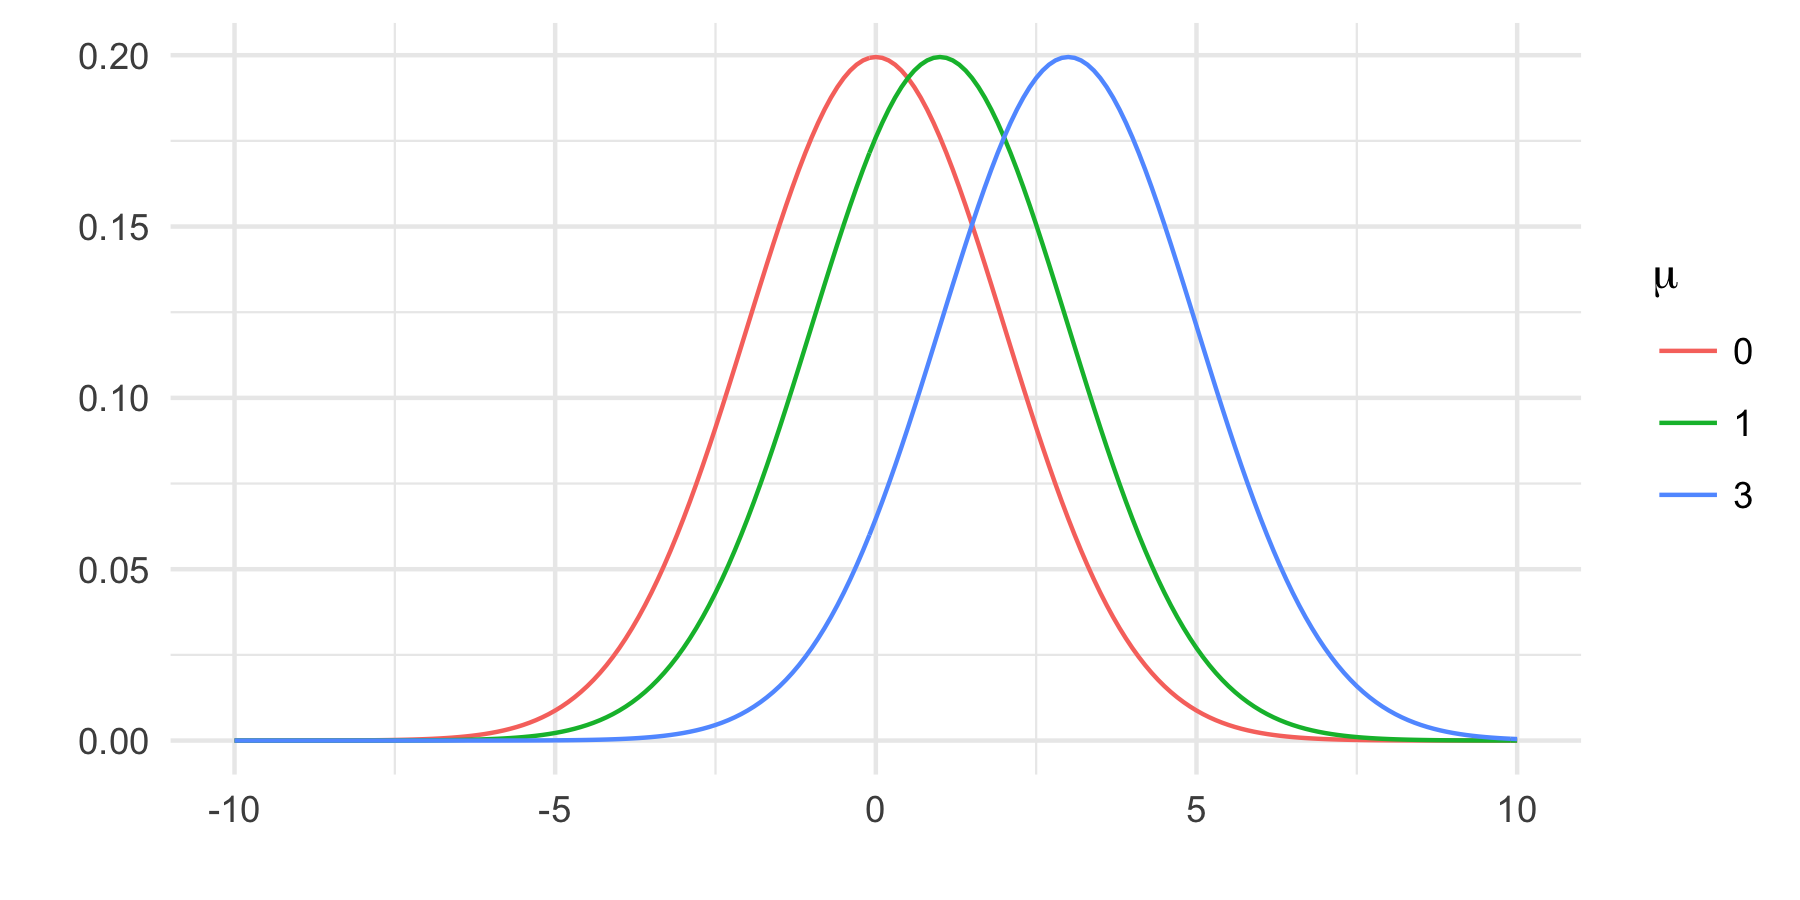
\includegraphics[width=0.9\textwidth]{img/l01-figure1a-normal-mean-change.png}
\end{center}
The value of $\sigma$ changes the width of the normal distribution.
\begin{center}
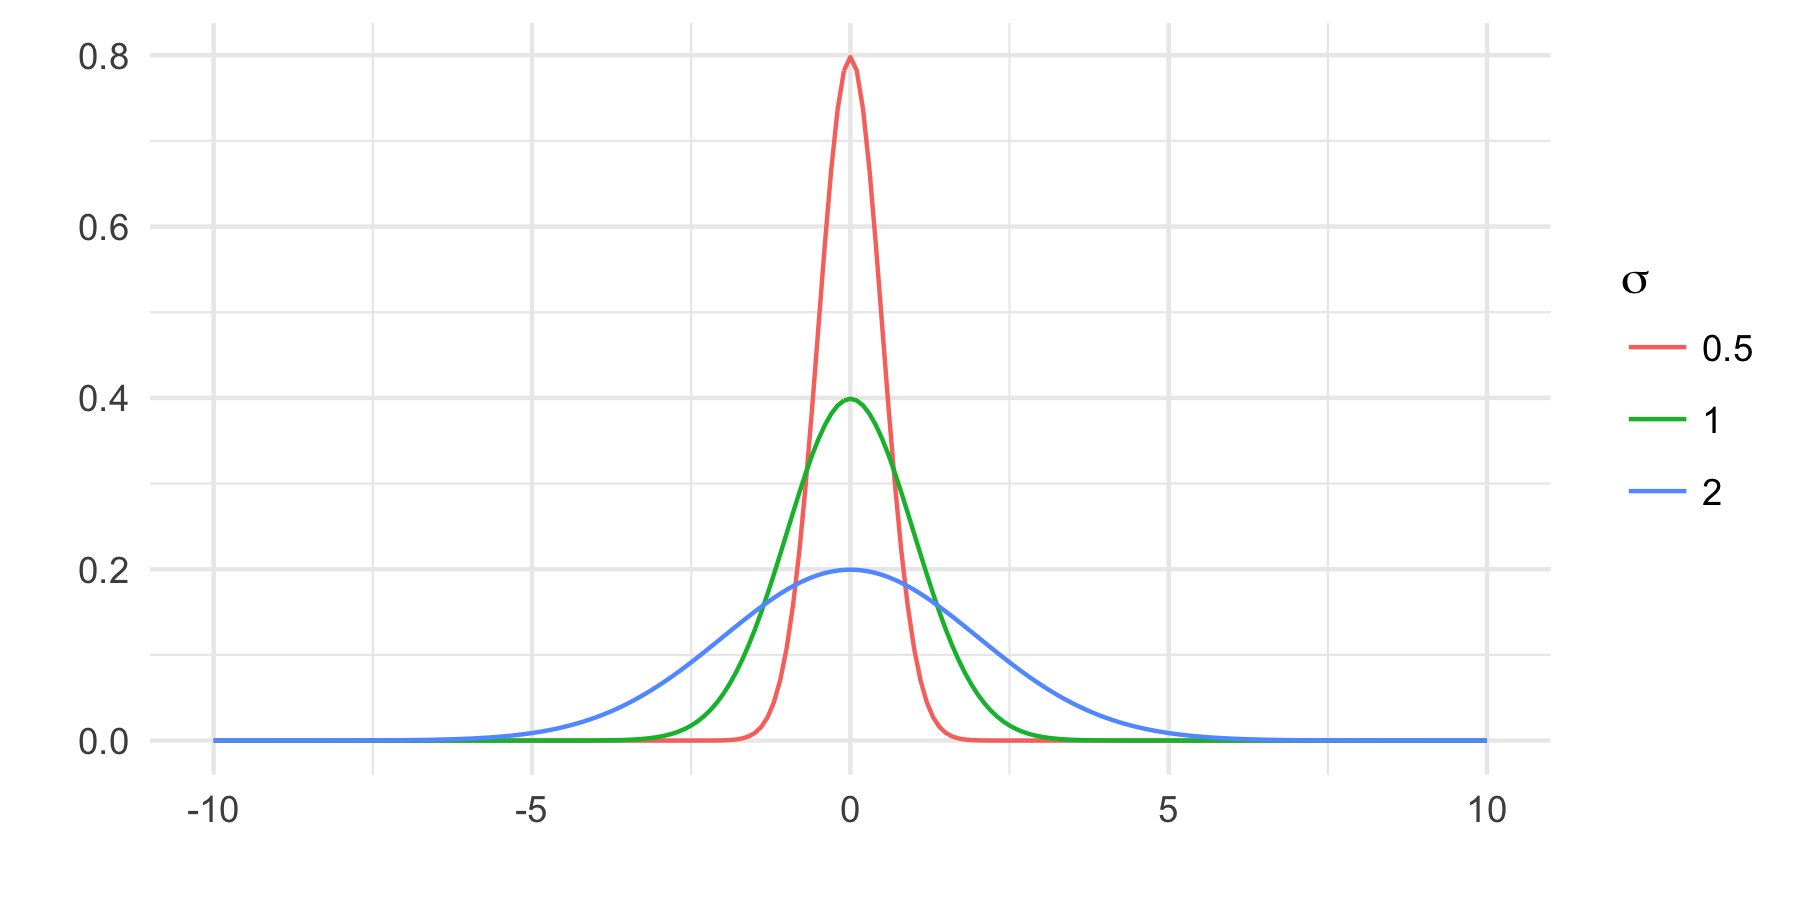
\includegraphics[width=0.9\textwidth]{img/l01-figure1b-normal-sd-change.png}
\end{center}

\begin{question}{}
List 5 random variables from medicine or biology that should follow normal distributions.
\end{question}
 

\section{Bernoulli Distribution}

The \textbf{Bernoulli distribution} is a discrete probability distribution with the following properties:
$$ p(x|\mu) = \mu^x (1 - \mu) ^ {1-x} \qquad E[x| \mu] = \mu \qquad \text{var}(x | \mu) = \mu (1 - \mu) $$
where $x \in \{0, 1\}$. It is used to model events where the outcome is yes/no. Think of it as a weighted coin, with $\mu$ the probability that the coin comes up ``heads'' on a single toss. Here are three Bernoulli distributions with (from left to right) $\mu = 1.0, 0.7, 0.2$. The number along the bottom is $x$, which can only be $0$ or $1$. 
\begin{center}
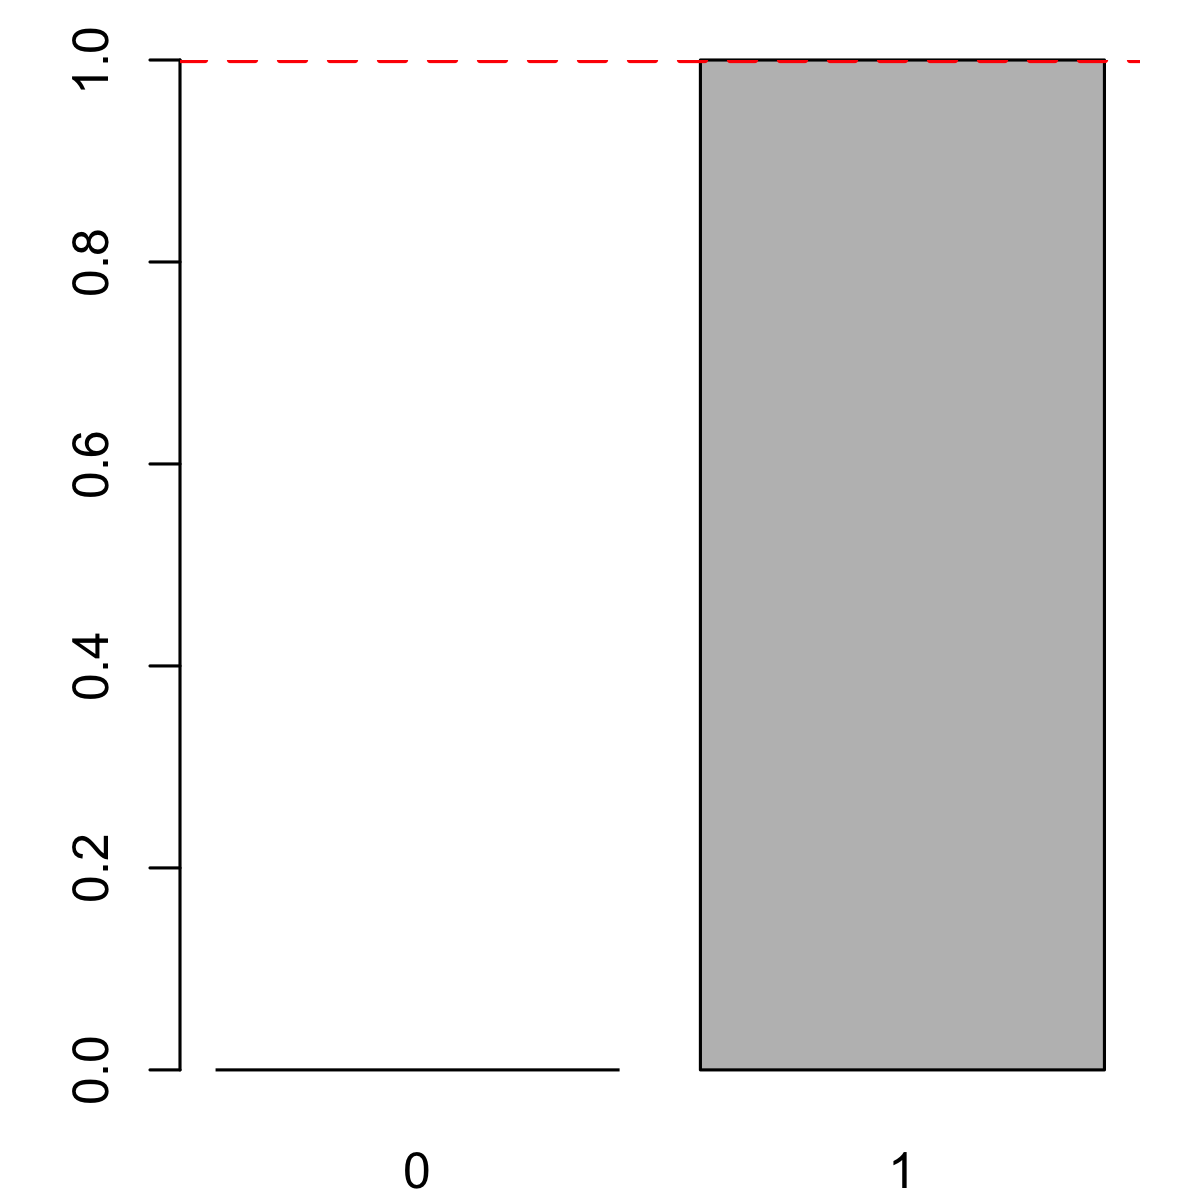
\includegraphics[width=0.3\textwidth]{img/l01-figure2a-bernoulli-1-0.png}
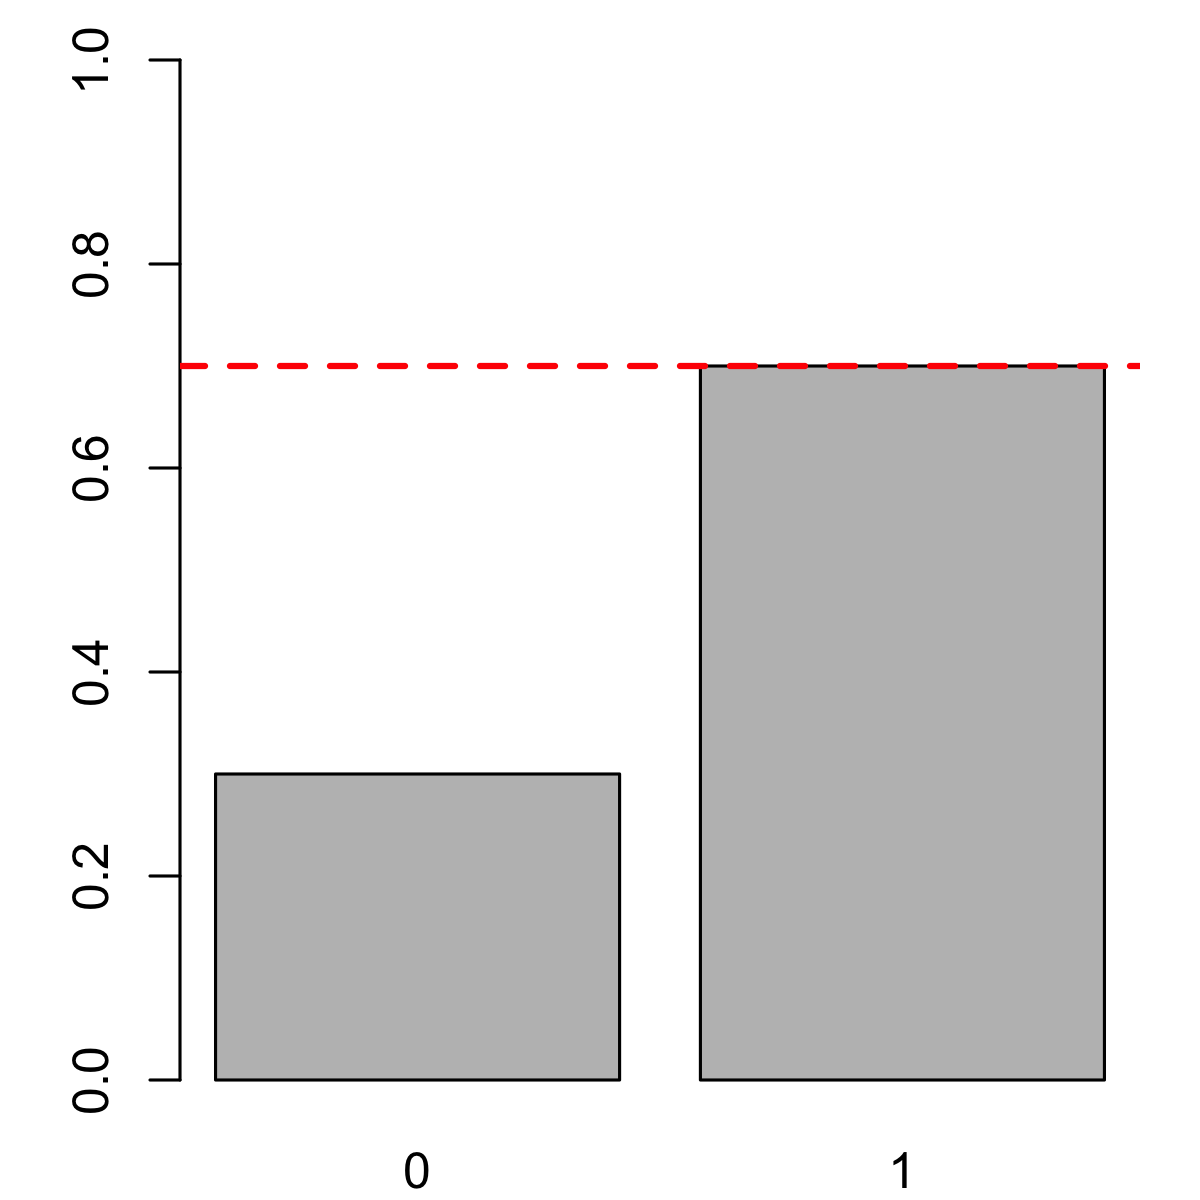
\includegraphics[width=0.3\textwidth]{img/l01-figure2b-bernoulli-0-7.png}
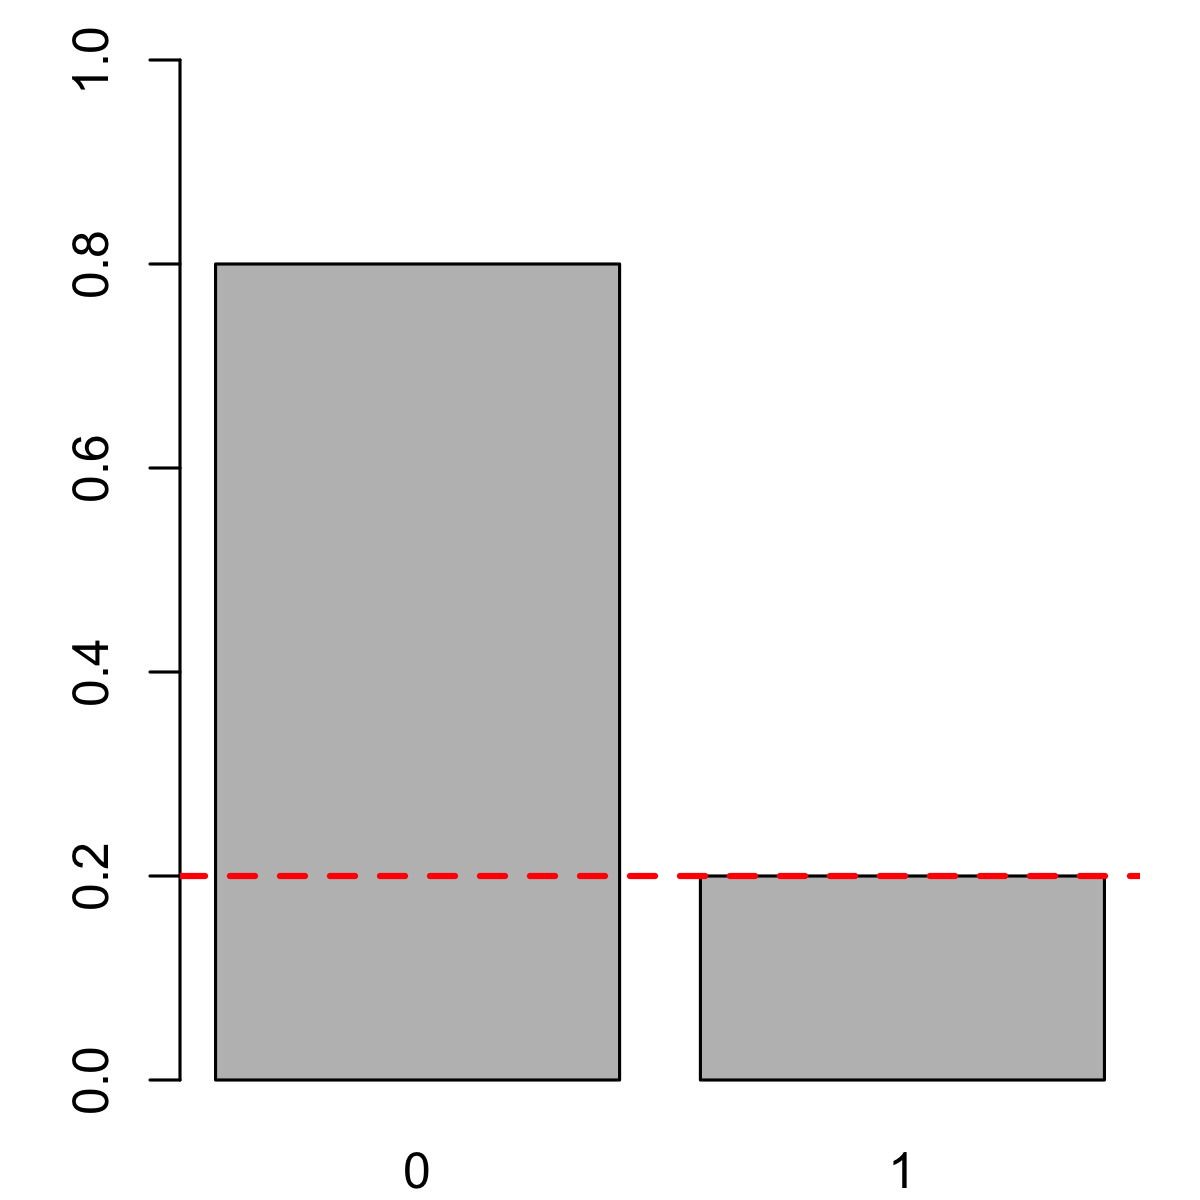
\includegraphics[width=0.3\textwidth]{img/l01-figure2c-bernoulli-0-2.png}
\end{center}

The \textbf{categorical distribution} is a generalization of the Bernoulli distribution to an outcome with more than two levels. The categorical distribution looks like this:
$$ p(x|\phi_1, \dots, \phi_K) = \phi_1^{\mathbb{I}(x=1)} \phi_2^{\mathbb{I}(x=2)} \cdots \phi_K^{\mathbb{I}(x=K)} $$
where $\sum_{k=1}^K \phi_k = 1$. The term $\mathbb{I}(x=j)$ is an \textbf{indicator}. It equals 1 if $x=j$ and 0 otherwise. For example, $\mathbb{I}(x=2)$ is 1 if $x=2$ and 0 otherwise. 

\begin{question}{}
List 5 random variables from medicine or biology that should follow Bernoulli distributions.
\end{question}


\section{Binomial Distribution}

The \textbf{binomial distribution} models the number of positive outcomes, $x$, out of $n$ independent\footnote{The word \textbf{independent} just means that the outcome of one trial does not influence the outcome of any other trial.} Bernoulli trials, each of which is positive with probability $\mu$. This distribution has the following properties, with $x \in \{0, \dots, n\}$:
$$ p(x|n,\mu) = {n\choose x} \mu^x (1 - \mu) ^ {n-x} \qquad E[x| \mu] = n \mu \qquad \text{var}(x | \mu) = n \mu (1 - \mu) $$
where the notation ${n \choose x}$ is defined as:
$$ {n \choose x} = \frac{n!}{x!(n-x)!}. $$
This notation denotes the number of ways it is possible to choose $x$ things out of a group of $n$ things, where the ordering doesn't matter. The exclamation point denotes the \textbf{factorial function}: $x! = x(x-1)(x-2)\cdots(2)(1)$. 

The shape of the binomial distribution is governed by the values of $n$ and $\mu$. Here, we vary $n$ but keep $\mu$ constant at $0.5$:
\begin{center}
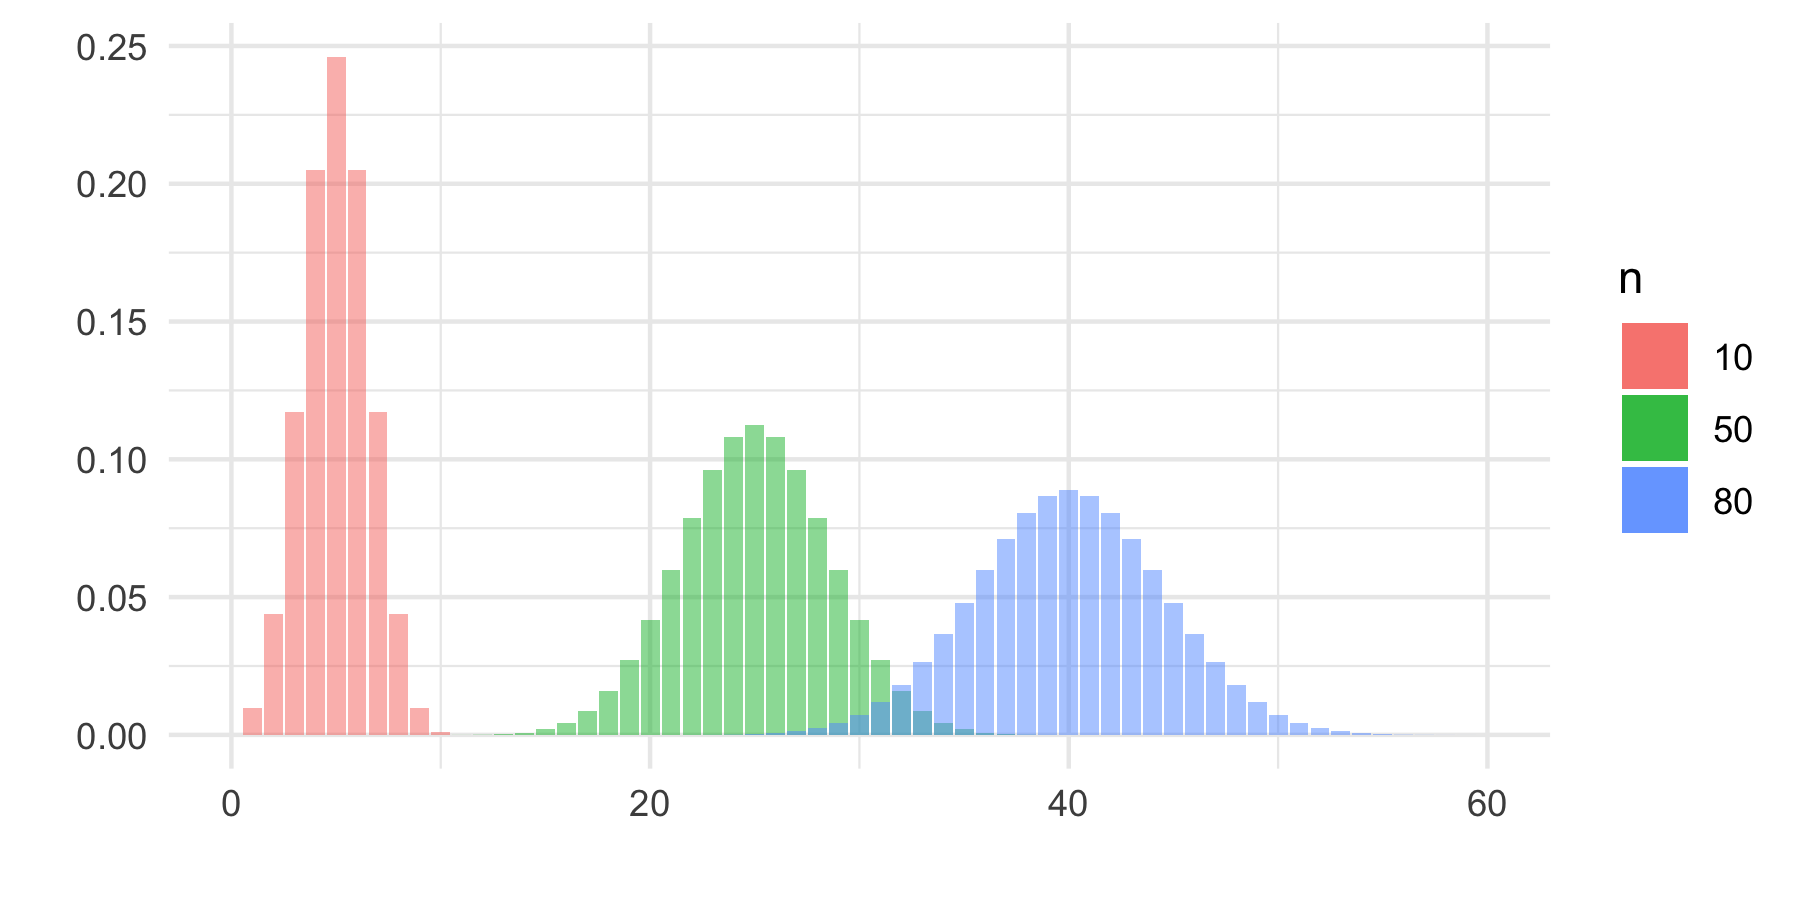
\includegraphics[width=0.9\textwidth]{img/l01-figure3-binom-n-change.png}
\end{center}
And here we vary $\mu$ but keep $n$ constant at $50$:
\begin{center}
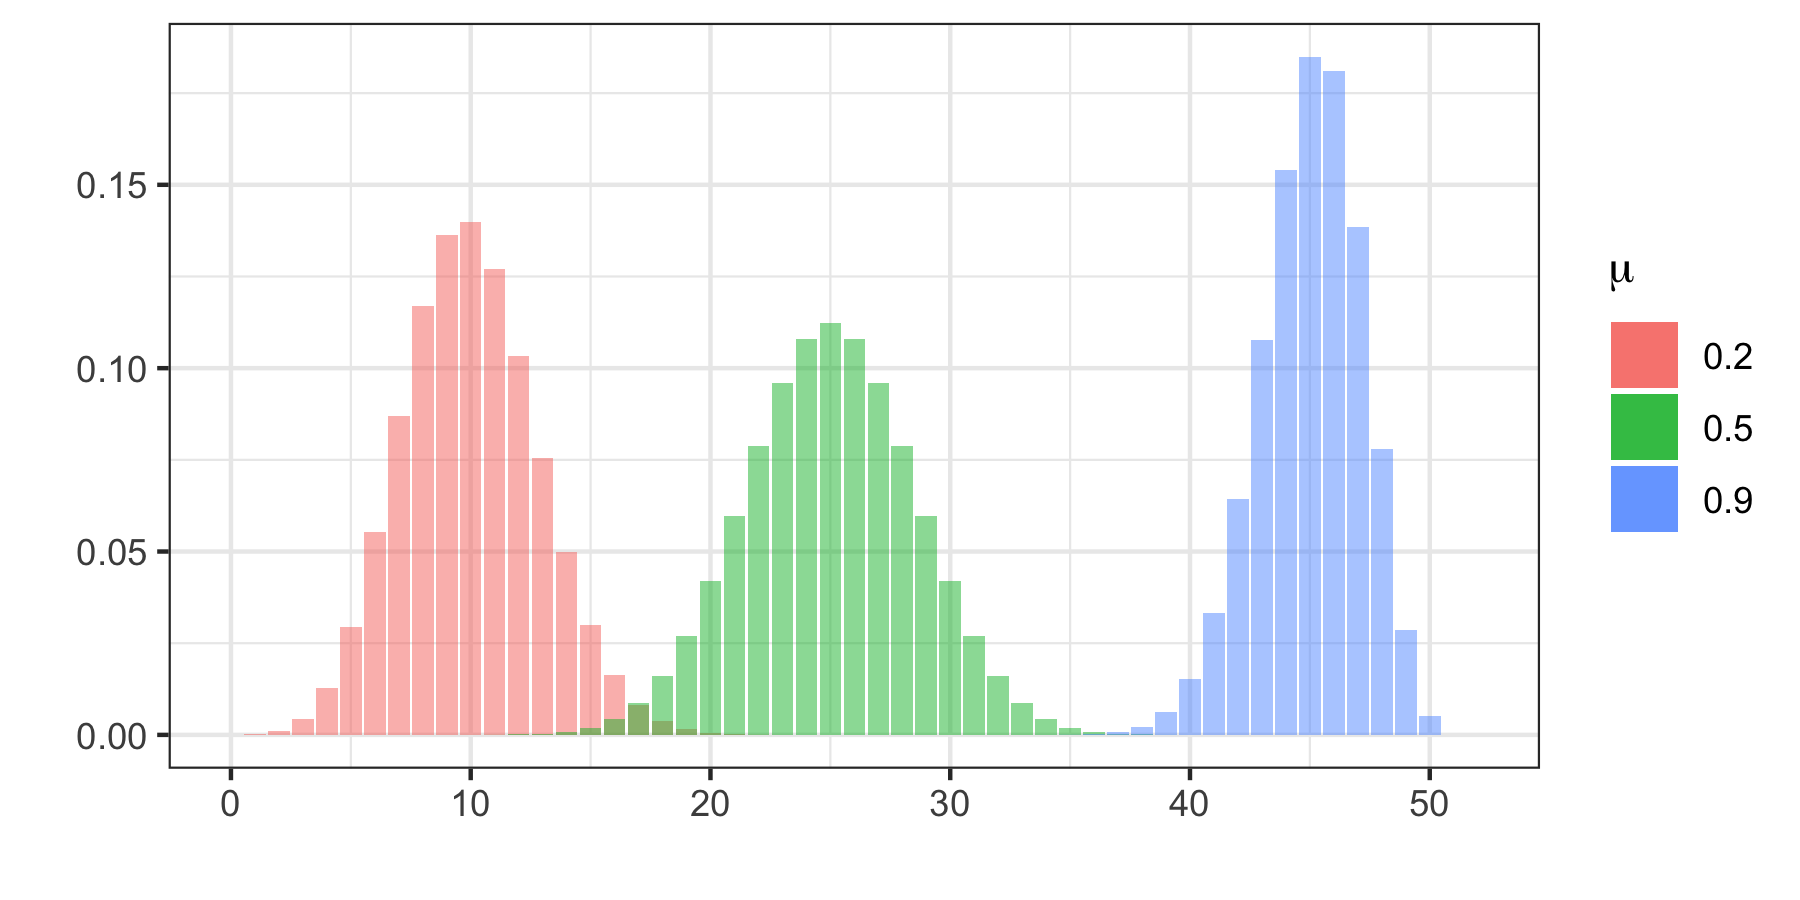
\includegraphics[width=0.9\textwidth]{img/l01-figure4-binom-p-change.png}
\end{center}

\begin{question}{}
List 5 random variables from medicine or biology that should follow binomial distributions.
\end{question}


\section{Poisson Distribution}

The \textbf{Poisson distribution} is a discrete probability distribution that is often used to model counts. It has the following properties:
$$ p(x | \lambda) = \frac{e^{-\lambda} \lambda^x}{x!} \qquad E[x|\lambda] = \lambda \qquad \text{var}(x|\lambda) = \lambda $$
where $x \in \left\{0, 1, 2, \dots \right\}$. Below are four examples of Poisson distributions. If events of a particular type occur continuously and independently at a constant rate (\textbf{Poisson process}), the number of events within a time window of fixed width will be distributed according to the Poisson distribution, with rate parameter $\lambda$ proportional to the width of the window.

\begin{center}
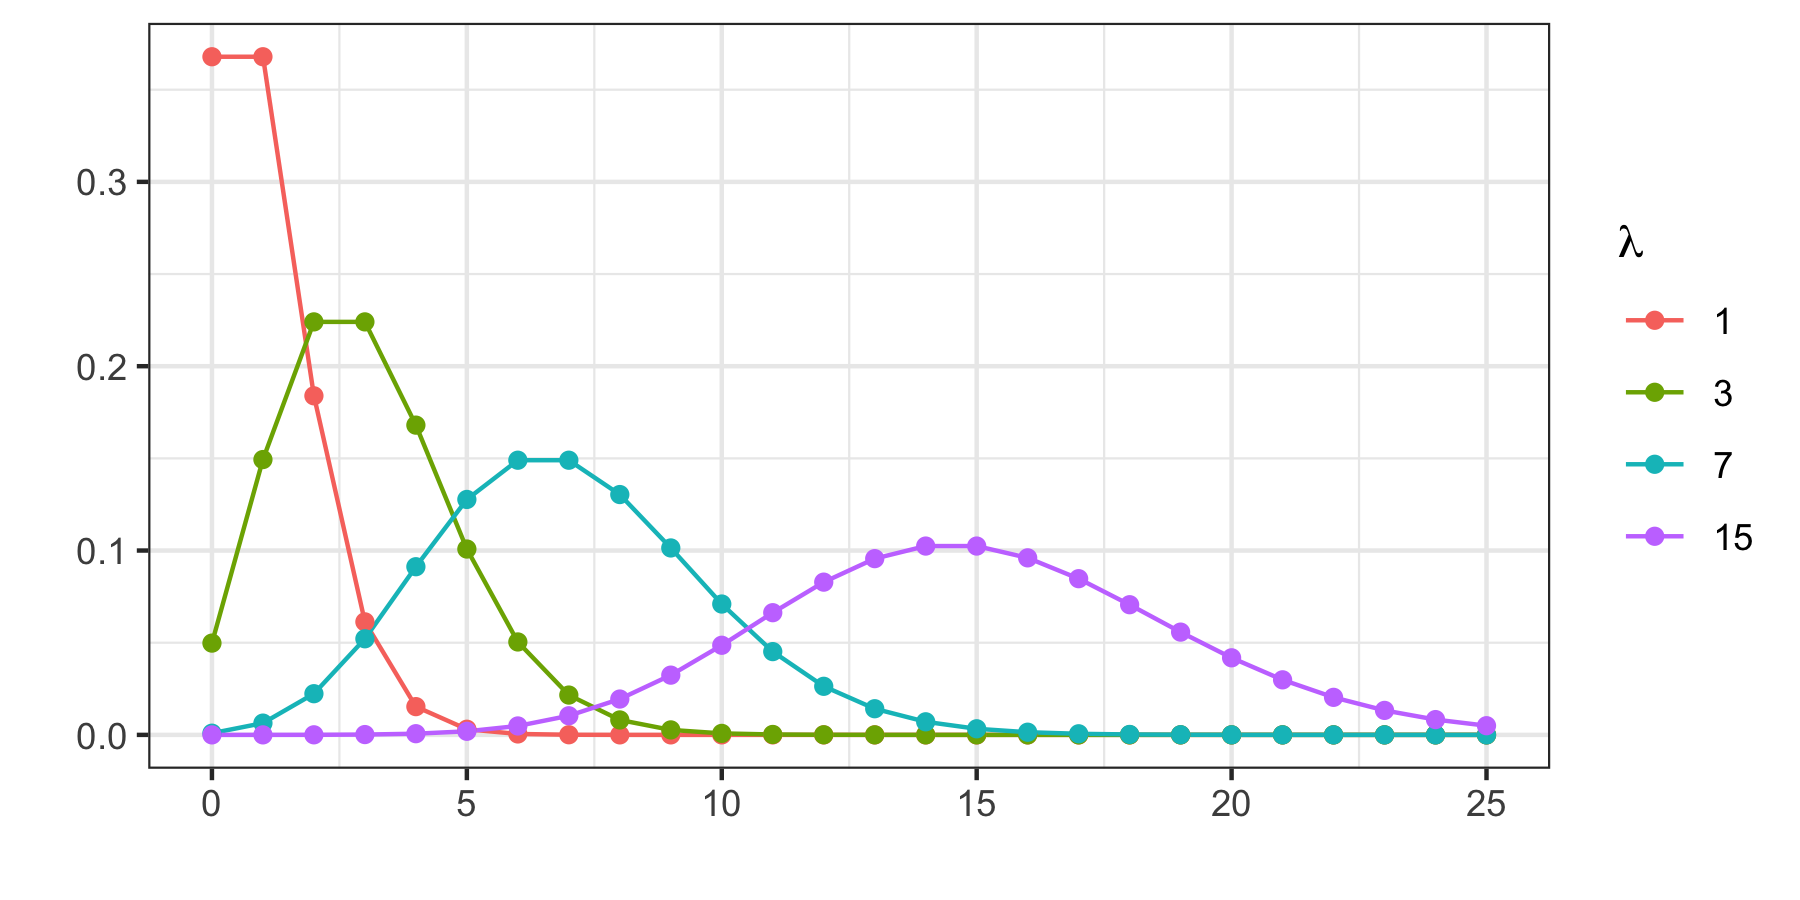
\includegraphics[width=0.9\textwidth]{img/l01-figure3a-poisson-lambda-change.png}
\end{center}

\begin{question}{}
List 5 random variables from medicine or biology that should follow Poisson distributions.
\end{question}


\section{Geometric}

The \textbf{geometric distribution} models the number of failures in a sequence of Bernoulli trials before the first success. It has the following properties:
$$ p(x|\mu) = (1-\mu)^x \mu \qquad E[x|\mu] = \frac{1-\mu}{\mu} \qquad \text{var}(x|\mu) = \frac{1-\mu}{\mu^2}  $$
for $x \in \left\{0, 1, 2, \dots \right\}$, where $\mu$ refers to the probability (in the Bernoulli trial) that the trial is a success. Some examples of geometric distributions with different $\mu$ are shown below: 
\begin{center}
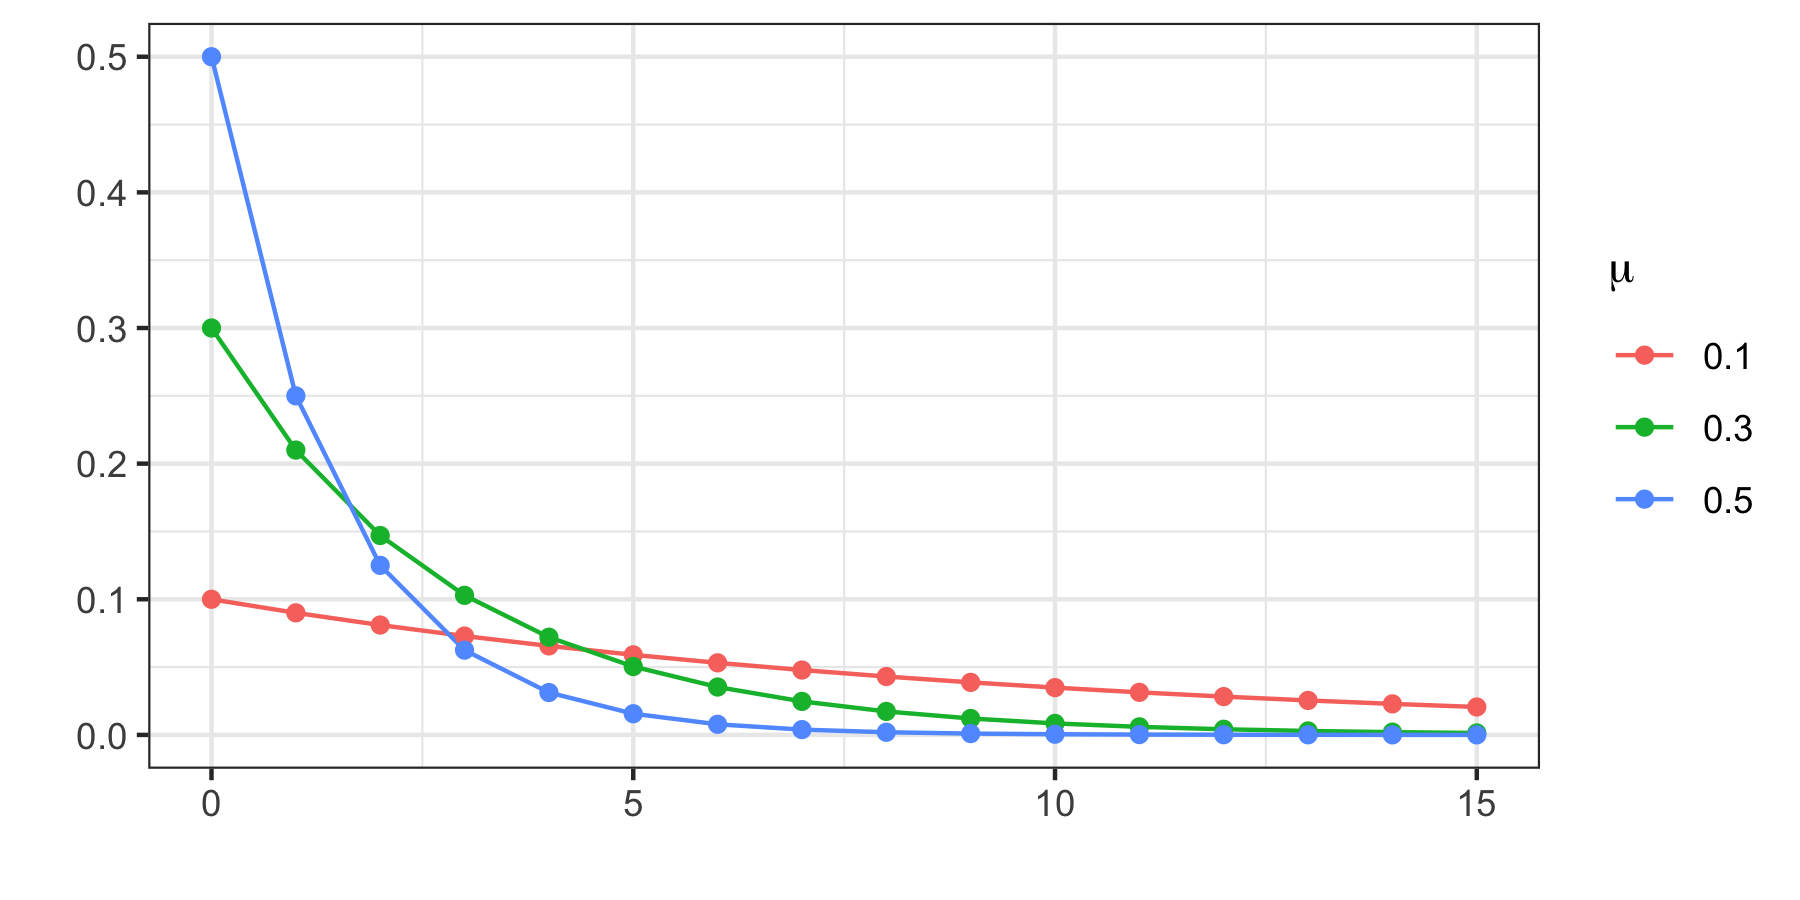
\includegraphics[width=0.9\textwidth]{img/l01-figure4-geometric-mu-change.png}
\end{center}

\begin{question}{}
List 5 random variables from medicine or biology that should follow Poisson distributions.
\end{question}


\section{Exponential}

The \textbf{exponential distribution} is a continuous probability distribution that models waiting times between events that happen independently and continuously at a constant rate (Poisson process), as well as many other random variables\footnote{For example, in an epidemiologic model of an infectious process like COVID-19 community spread, exponential waiting times are often used to model transitions between the susceptible, exposed, infectious, and recovered compartments in the model.}. It has the following properties:
$$ p(x|\lambda) = \lambda e^{-\lambda x} \qquad E[x|\lambda] = \frac{1}{\lambda} \qquad \text{var}(x|\lambda) = \frac{1}{\lambda^2} $$
where $x \in \mathbb{R}^+$ ($x$ is a positive real number, or zero). The exponential distribution is the continuous analogue of the geometric distribution. It is memoryless, which means that the distribution of a waiting time until an event does not depend on how much time has elapsed already.

Here are some different exponential distributions. Compare them to the geometric distribution, above.
\begin{center}
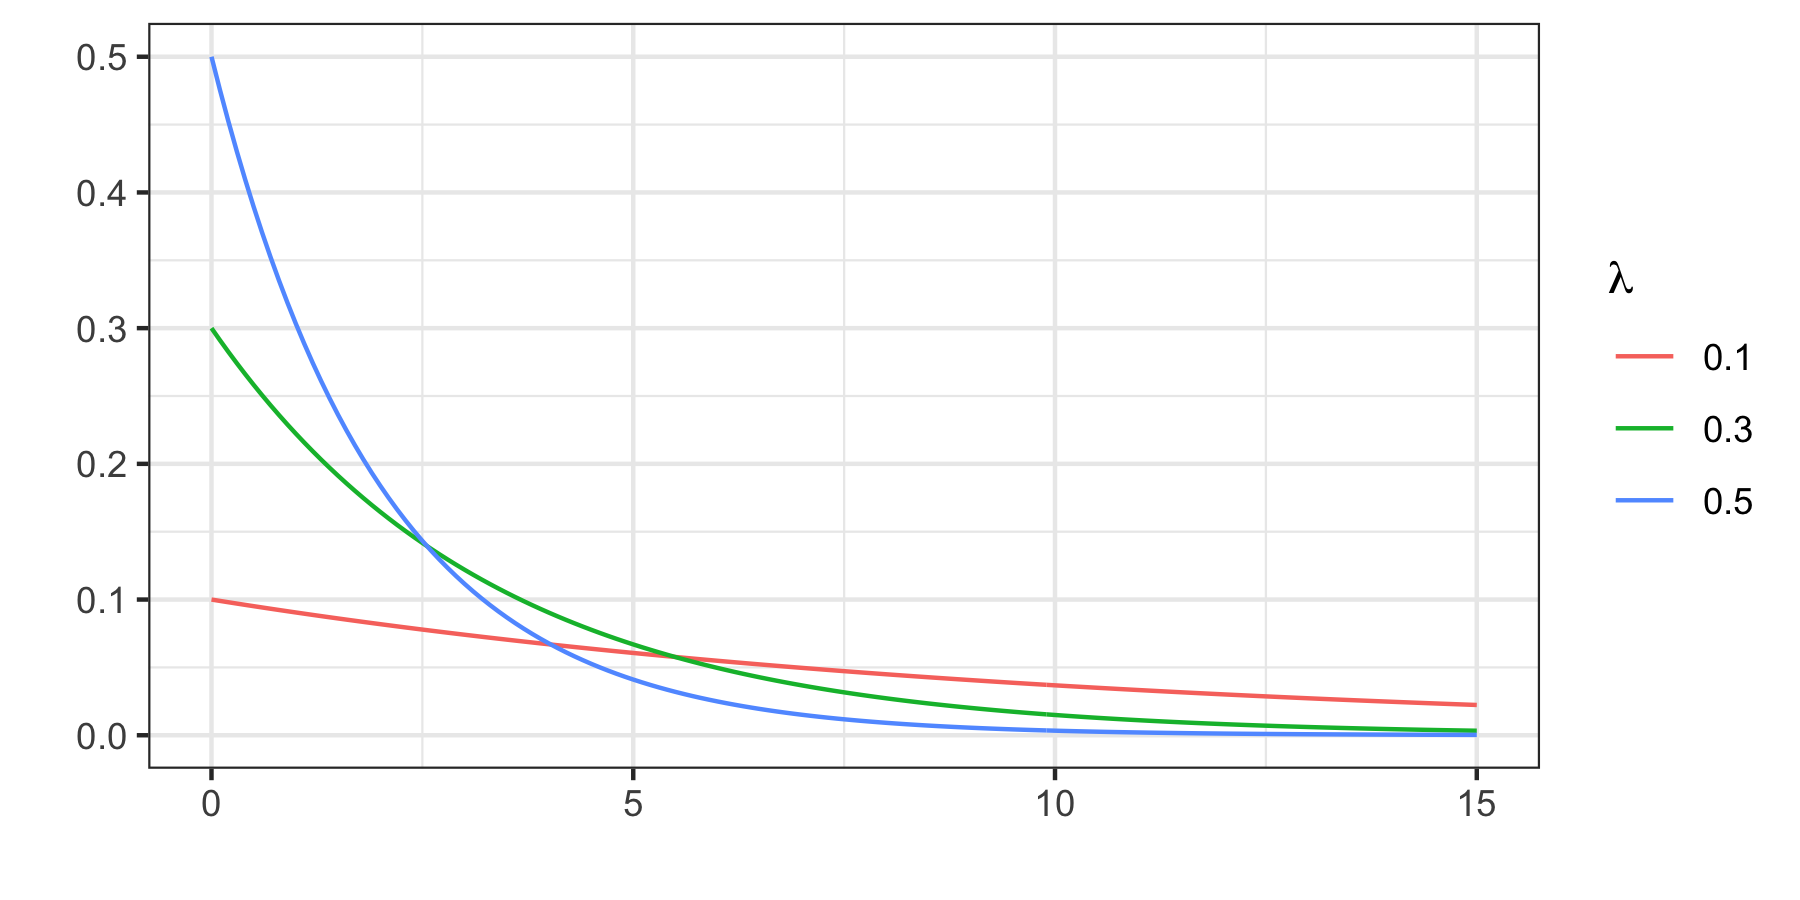
\includegraphics[width=0.9\textwidth]{img/l01-figure5-exponential-lambda-change.png}
\end{center}

\begin{question}{}
List 5 random variables from medicine or biology that should follow exponential distributions.
\end{question}


\section{Chi-Squared Distribution}

How this distribution arises:
\begin{enumerate}
\item If $Z \sim \mathcal{N}(0, 1)$, the distribution of $U = Z^2$ is called the chi-squared distribution with one degree of freedom.
\item If $U_1, U_2, \dots, U_k$ are independent $\chi_1^2$ random variables, their sum,
$ V = \sum_{i=1}^k U_i $
follows $\chi_k^2$, a chi-squared distribution with $k$ degrees of freedom.
\end{enumerate}

You'll often see the chi-squared distribution used as the sampling distribution for the sample variance in a variety of statistical hypothesis tests. It looks like this:
\begin{center}
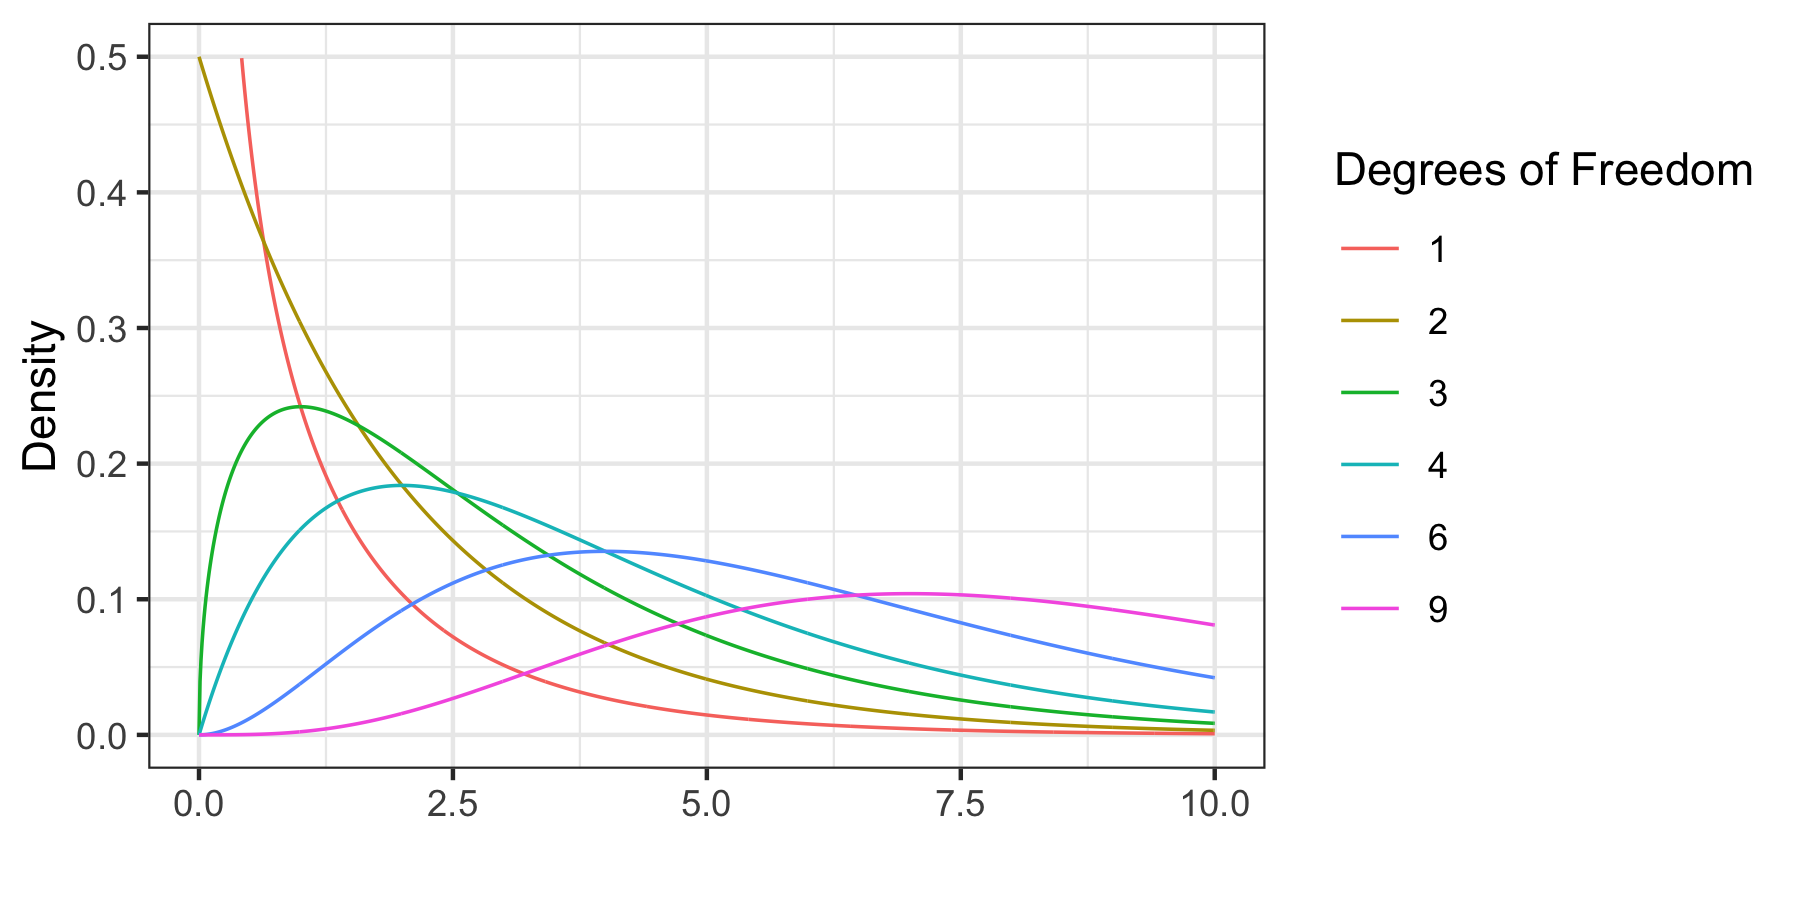
\includegraphics[width=0.9\textwidth]{img/hyp-example-chisq-distribution.png}
\end{center}

The parameter $k$, the \textbf{degrees of freedom}, controls the shape of the chi-squared distribution. The actual formula for the chi-squared distribution looks a bit intimidating, but I'm including it here so you can compare it to the other distributions we've seen:
$$ p(x|k) = \frac{1}{2^{k/2} \Gamma(k/2)} x^{k/2 - 1} e^{-x/2} $$
$$ E[x | k] = k \qquad \text{var}(x | k) = 2k $$ 
The gamma function shown in the denominator of the probability density,
$$ \Gamma(z) = \int_0^{\infty} x^{z-1} e^{-x} dx, $$
is a generalization of the factorial function to complex numbers. For any positive integer $n$, $\Gamma(n) = (n-1)!$. 

\section{Student's T Distribution}

If $Z \sim \mathcal{N}(0, 1)$ and $U \sim \chi_k^2$ and $Z$ and $U$ are independent, 
$$ T = \frac{Z}{\sqrt{U/k}} \sim t_k $$
or in words, the statistic $T$ follows a $t$-distribution with $k$ degrees of freedom. The T distribution plays an important role in a family of statistical hypothesis tests called T-tests. 

\begin{center}
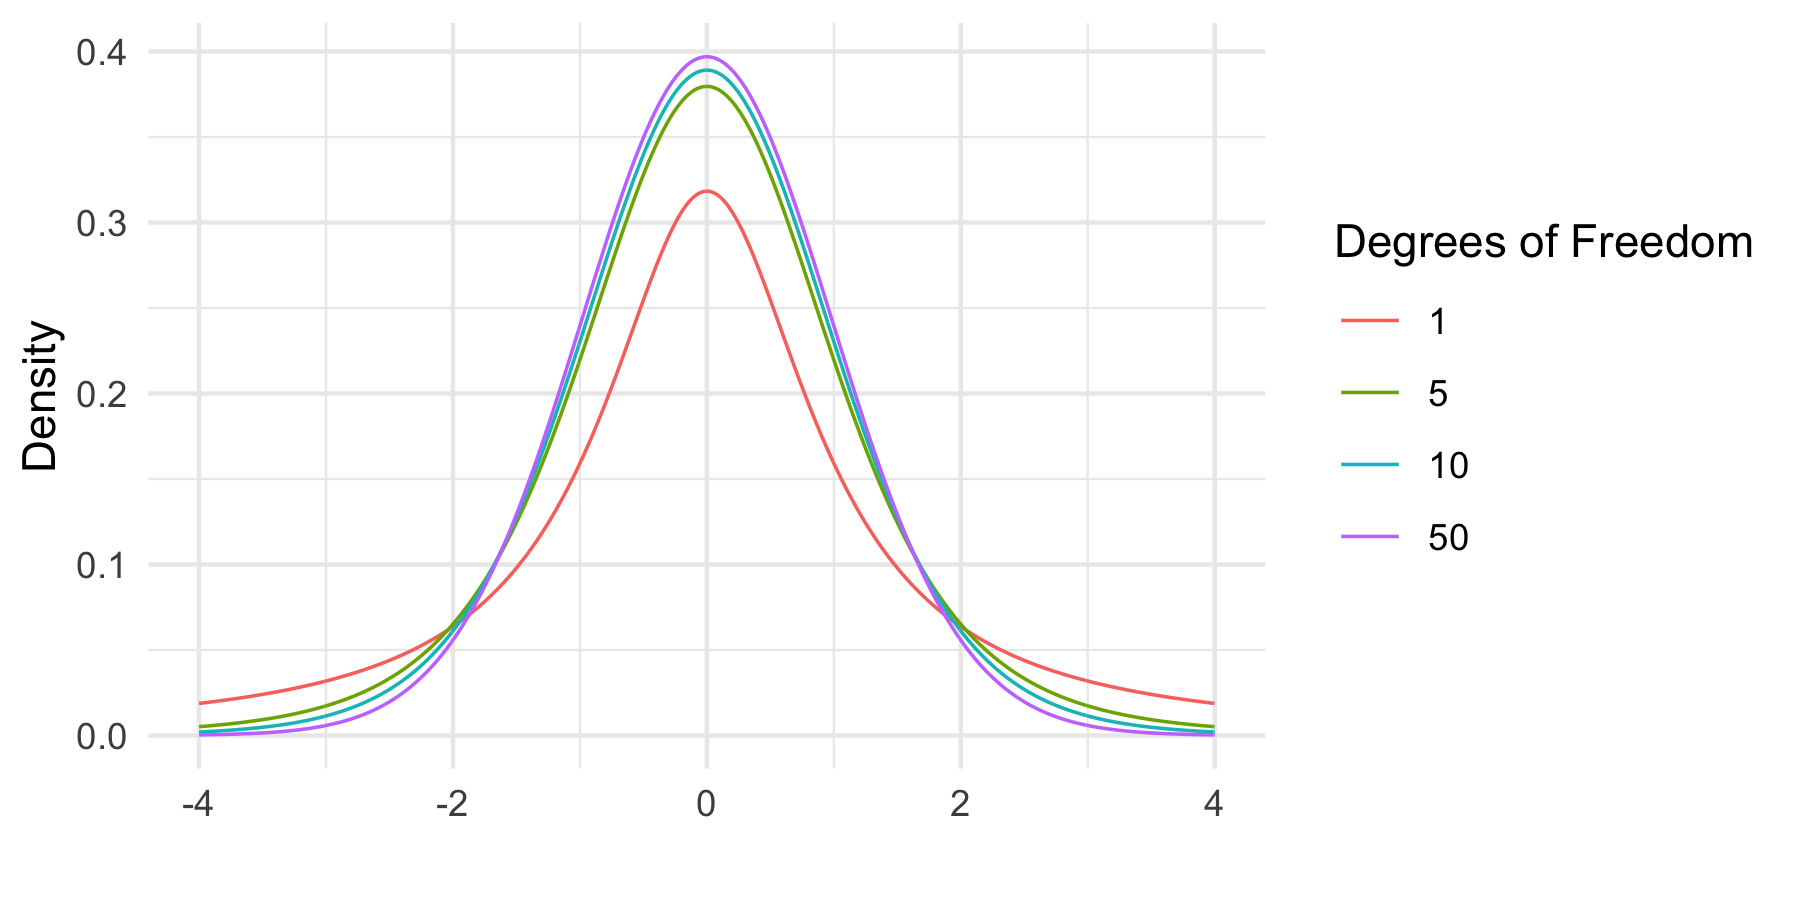
\includegraphics[width=0.9\textwidth]{img/hyp-example-t-distribution.png}
\end{center}

Again, the functional form of the T distribution is a bit intimidating, but I'm including it for completeness:

$$ p(x|k) = \frac{\Gamma \left(\frac{k+1}{2} \right)} {\sqrt{k\pi}\,\Gamma \left(\frac{k}{2} \right)} \left(1+\frac{x^2}{k} \right)^{-\frac{k+1}{2}} $$
$$ E[x|k] = 0~~\text{ for }k>1; \text{ otherwise undefined} $$
$$ \text{var}(x|k) = \left\{ \begin{array}{cl} \frac{k}{k-2} & k>2 \\
                                               \infty & 1 < k \leq 2 \\
                                               \text{undefined} & \text{otherwise} \end{array} \right. $$

\section{F Distribution}

If $U$ and $V$ are independent $\chi^2$ random variables with $m$ and $n$ degrees of freedom,
$$ W = \frac{U/m}{V/n} \sim F_{m, n} $$
or in words, the statistic $W$ follows an $F$ distribution with $m$ and $n$ degrees of freedom. I'm not writing out the functional form of the F distribution here because it's too awful-looking, but graphically it looks like this:
\begin{center}
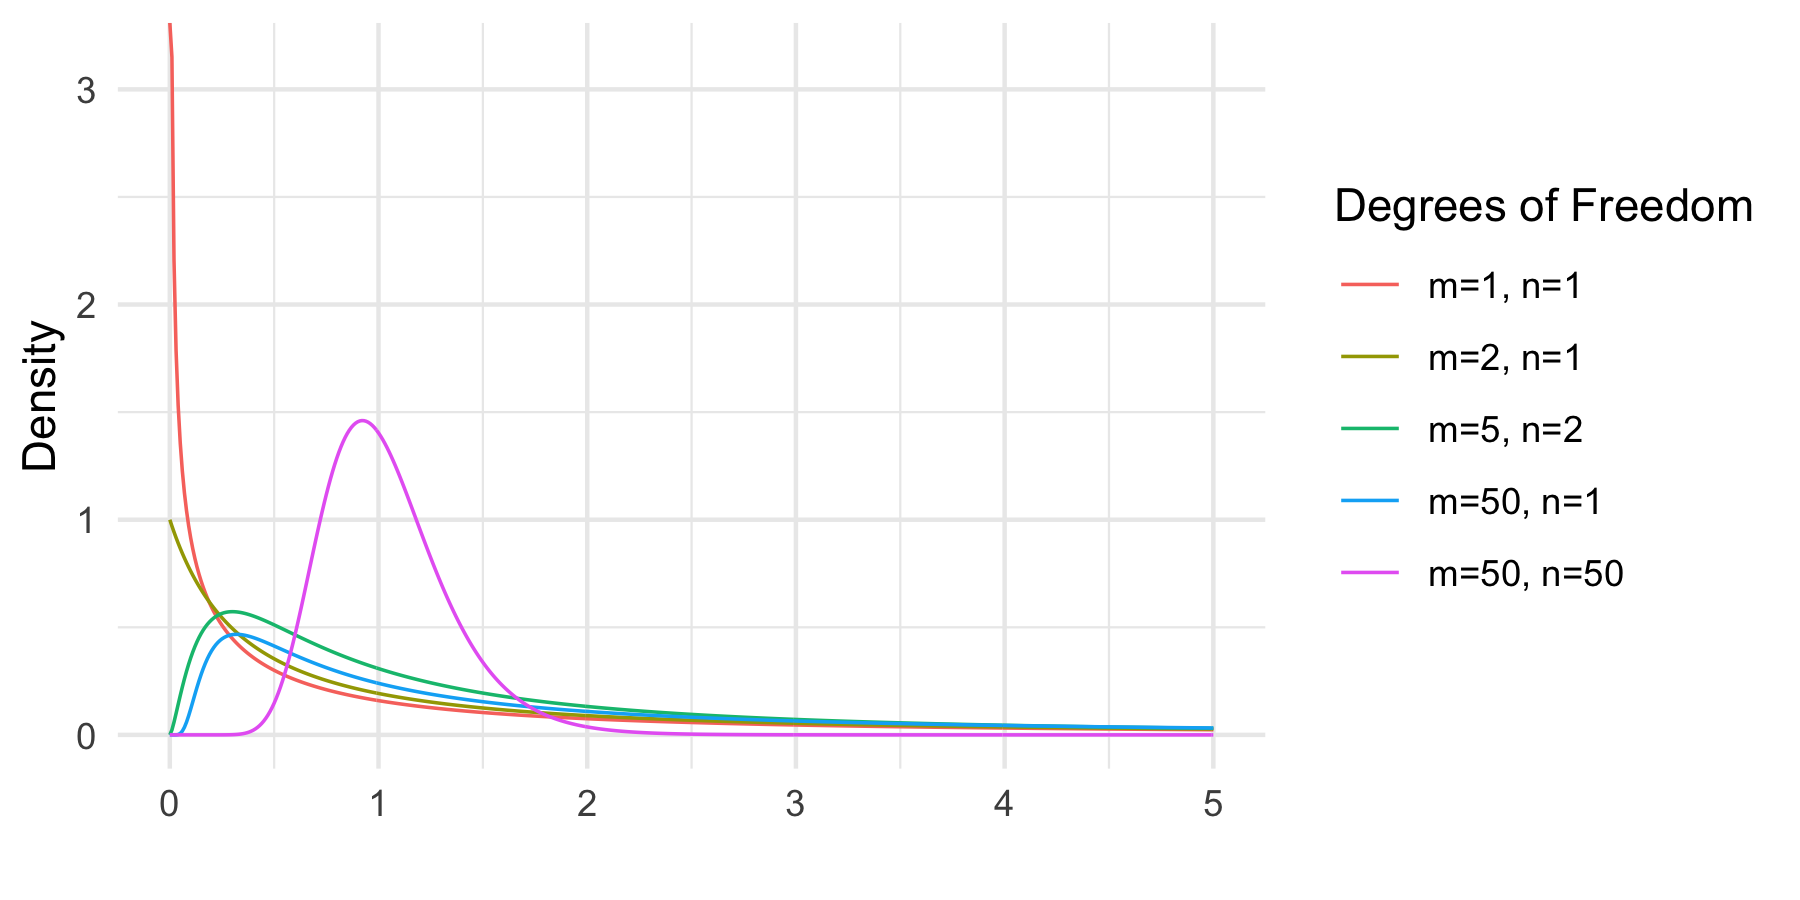
\includegraphics[width=0.9\textwidth]{img/hyp-example-f-distribution.png}
\end{center}

Note that if $T \sim t_k$, then $T^2 \sim F_{1,k}$. The $F$-distribution plays an important role in a class of statistical analysis techniques called \textbf{ANalysis Of VAriance}, or \textbf{ANOVA}.

\vspace{2mm}

\begin{question}{}
For each of the following experimental conditions, which distribution (from those listed above) provides the best model for how the data $x^{(1)},\dots,x^{(n)}$ are generated?
    \begin{enumerate}
    \item[(a)] You are observing several patients' skin in a clinical study to see how long it takes them to develop a rash. You take a picture each day. Let $x^{(i)}$ be the number of days of \emph{no rash} before the rash occurs.

\begin{center}{\small
\begin{tabular}{cc}
\toprule
Patient ID ($i$) & $x^{(i)}$ \\
\midrule
1 & 4 \\
2 & 1 \\
3 & 0 \\
4 & 2 \\
5 & 2 \\
6 & 4 \\
7 & 3 \\
8 & 1 \\
9 & 0 \\
10 & 1 \\
\end{tabular}}
\end{center}

    \item[(b)] Same situation as above except that instead of taking a picture each day, the patient texts you at the moment he/she observes a rash. The data look like this, where $x^{(i)}$ is the time (in days) at which patient $i$ develops a rash: 

\begin{center}{\small
\begin{tabular}{cc}
\toprule
Patient ID ($i$) & $x^{(i)}$ \\
\midrule
1 & 2.25 \\
2 & 3.43\\
3 & 0.68\\
4 & 0.04\\
5 & 3.78\\
6 & 5.65\\
7 & 2.88\\
8 & 3.88\\
9 & 2.83\\
10 & 1.87\\
\end{tabular}}
\end{center}
 
    \item[(c)] Imagine you are Ladislaus Bortkiewicz, and you are modeling the number of persons killed by mule or horse kicks in the Prussian army per year. You have data from the late 1800s over the course of 20 years. Let $x^{(i)}$ be the number of people killed in year $i$.
        
\begin{center}{\small
\begin{tabular}{cc|cc}
\toprule
Year ($i$) & $x^{(i)}$ & Year ($i$) & $x^{(i)}$ \\
\midrule
1 & 8 & 11 & 9 \\
2 & 10 & 12 & 7 \\
3 & 5 & 13 & 10 \\
4 & 3 & 14 & 12 \\
5 & 10 & 15 & 8 \\
6 & 8 & 16 & 7 \\
7 & 7 & 17 & 8 \\
8 & 2 & 18 & 8 \\
9 & 6 & 19 & 10 \\
10 & 11 & 20 & 7 \\
\end{tabular}}
\end{center}
    
    \item[(d)] Every year, $10$ scientists go to the same geographic area (same Lyme prevalence) and they each collect $40$ ticks. They test each tick for Lyme disease and record the number of ticks that have Lyme. Let $x^{(i)}$ be the number of ticks with Lyme in the $i$th scientist's bunch.
        
\begin{center}{\small
\begin{tabular}{cc}
\toprule
Scientist ID ($i$) & $x^{(i)}$ \\
\midrule
1 & 8 \\
2 & 9 \\
3 & 14 \\
4 & 15 \\
5 & 12 \\
6 & 7 \\
7 & 6 \\
8 & 8 \\
9 & 8 \\
10 & 14 \\
\end{tabular}}
\end{center}
    
    \item[(e)] You have waist circumference data on 1045 men aged 70 and above (see Dey's 2002 paper in the Journal of the American Geriatric Society). It looks like this:
    
\begin{center}
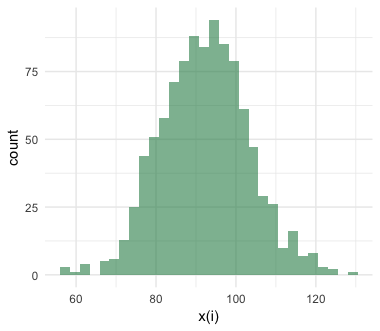
\includegraphics[width=0.5\textwidth]{img/l01-problem5.png}
\end{center}

    \end{enumerate}
\end{question}

